\documentclass{standalone}

\usepackage{tikz}
\usetikzlibrary{shapes, arrows}
\usetikzlibrary{arrows,calc,decorations.markings,math,arrows.meta}
\usetikzlibrary{positioning}
\usepackage{graphicx}



\begin{document}
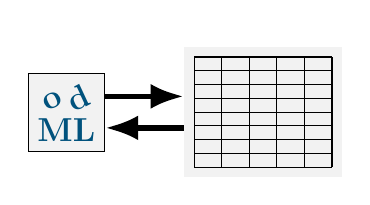
\begin{tikzpicture}
		    \definecolor{odmlcolor}{rgb}{0.00,0.32,0.49}
		    \definecolor{back}{rgb}{0.95,0.95,0.95}
		    \node(odml) [draw,align=center,font=\bfseries,fill=back]{\large \textcolor{odmlcolor}{\rotatebox[origin=c]{25}{o}\rotatebox[origin=c]{25}{d}} \\ \large{\textcolor{odmlcolor}{ML}}};
		    \node[right = 1cm of odml,fill=back] (table) {\tikz{
		    \begin{scope}[scale=0.35]
		      \draw[xstep=1,ystep=0.5] (-2,-2) grid (3,2);
		    \end{scope}
		    }};
		    
		    \node[above = 0cm of table](tabletext) {};
		    
		    \draw[-{Latex[scale=1]},line width=0.7mm] ([yshift=0.2cm]odml.east) -- ([yshift=0.2cm]table.west) {};
		    \draw[{Latex[scale=1]}-,line width=0.7mm] ([yshift=-0.2cm]odml.east) -- ([yshift=-0.2cm]table.west) {};
\end{tikzpicture}
\end{document}
